\documentclass{beamer}
\usepackage[dvipsnames]{xcolor}
\usepackage{listings}
\usepackage{graphicx}
\usepackage{tikz}
\usepackage{xcolor}

\setbeamertemplate{navigation symbols}{}
\usetheme{Madrid}

\definecolor{kotlin-purple}{HTML}{7F52FF}
\definecolor{redhighlight}{RGB}{255,200,200}
\definecolor{greenhighlight}{RGB}{200,255,200}


\iffalse %wird bis \fi ignoriert
% Brighter, cohesive color scheme
\definecolor{bgcolor}{HTML}{E8F1FB}
\definecolor{bgcoloralt}{HTML}{F2F4F7}
\definecolor{basecolor}{HTML}{60A5FA}
\definecolor{secondarycolor}{HTML}{93C5FD}
\definecolor{textcolor}{HTML}{1E293B}
\definecolor{popcolor}{HTML}{FCD34D}
\definecolor{bgpopcolor}{HTML}{FFF7ED}


% altcolor scheme
\definecolor{altbgcolor}{HTML}{FFF7ED}
\definecolor{altbgcoloralt}{HTML}{FEFCF8}
\definecolor{altbasecolor}{HTML}{6B7280}
\definecolor{altsecondarycolor}{HTML}{D1D5DB}
\definecolor{alttextcolor}{HTML}{1F2937}
\definecolor{altpopcolor}{HTML}{8054FC}

%thread colors
%\definecolor{main}{HTML}{60A5FA}  % Red → Blue
\definecolor{defaultcolor}{HTML}{C084FC}  % Yellow → Violet
\definecolor{iocolor}{HTML}{A3E635}  % Blue → Lime Green
%thread colors
%\definecolor{main}{HTML}{60A5FA}  % Red → Blue
\definecolor{defaultcolor}{HTML}{C084FC}  % Yellow → Violet
\definecolor{iocolor}{HTML}{A3E635}  % Blue → Lime Green

\definecolor{altbasecolor}{HTML}{8054FC}  % Red shifted → Violet

\fi

% color scheme

\definecolor{bgcolor}{HTML}{EDE9FB}
\definecolor{bgcoloralt}{HTML}{F4F4F7}
\definecolor{bgpopcolor}{HTML}{FFF7ED}
\definecolor{basecolor}{HTML}{8054FC}
\definecolor{secondarycolor}{HTML}{B69DFD}
\definecolor{textcolor}{HTML}{1E1B2E}
\definecolor{popcolor}{HTML}{FBBF24}



% altcolor scheme

\definecolor{altbgcolor}{HTML}{E0E7FF}
\definecolor{altbgcoloralt}{HTML}{D1D5DB}
\definecolor{altbasecolor}{HTML}{334155}
\definecolor{altsecondarycolor}{HTML}{94A3B8}
\definecolor{alttextcolor}{HTML}{1E293B}
\definecolor{altpopcolor}{HTML}{EDE9FB}

%thread colors
\definecolor{defaultcolor}{HTML}{FB61B4}
\definecolor{iocolor}{HTML}{6EE7B7}  





\lstdefinelanguage{Kotlin}{
  comment=[l]{//},
  morecomment=[s]{/*}{*/},
  emph={filter, first, firstOrNull, forEach, lazy, map, mapNotNull, println},
  keywords={!in, !is, abstract, actual, annotation, as, as?, break, by, catch, class, companion, const, constructor, continue, crossinline, data, delegate, do, dynamic, else, enum, expect, external, false, field, file, final, finally, for, fun, get, if, import, in, infix, init, inline, inner, interface, internal, is, lateinit, noinline, null, object, open, operator, out, override, package, param, private, property, protected, public, receiveris, reified, return, return@, sealed, set, setparam, super, suspend, tailrec, this, throw, true, try, typealias, typeof, val, var, vararg, when, where, while},
  ndkeywords={@Deprecated, @JvmField, @JvmName, @JvmOverloads, @JvmStatic, @JvmSynthetic, Array, Byte, Double, Float, Int, Integer, Iterable, Long, Runnable, Short, String, Any, Unit, Nothing},
  morestring=[b]",
  morestring=[s]{"""*}{*"""},
  sensitive=true,
  moredelim=[is][\hlg]{<g>}{</g>},
  moredelim=[is][\hlr]{<r>}{</r>},
  moredelim=[is][\hlgBlue]{<gBlue>}{</gBlue>},
  moredelim=[is][\hlrBlue]{<rBlue>}{</rBlue>},
}

\lstdefinelanguage{Java}{
  comment=[l]{//},
  morecomment=[s]{/*}{*/},
  emph={System, out, print, println, Arrays, Collections, List, Map, Set, stream},
  keywords={abstract, assert, boolean, break, byte, case, catch, char, class, const, continue, default, do, double, else, enum, extends, final, finally, float, for, if, goto, implements, import, instanceof, int, interface, long, native, new, null, package, private, protected, public, return, short, static, strictfp, super, switch, synchronized, this, throw, throws, transient, try, void, volatile, while, var},
  ndkeywords={@Deprecated, @FunctionalInterface, @Override, @SafeVarargs, @SuppressWarnings, @Documented, @Inherited, @Repeatable, @Retention, @Target, String, Integer, Double, Float, Long, Short, Boolean, Character, Object, Class, Runnable},
  morestring=[b]",
  morestring=[s]{"""*}{*"""},
  sensitive=true,
  moredelim=[is][\hlg]{<g>}{</g>},
  moredelim=[is][\hlr]{<r>}{</r>},
  moredelim=[is][\hlgBlue]{<gBlue>}{</gBlue>},
  moredelim=[is][\hlrBlue]{<rBlue>}{</rBlue>},
}

\newcommand{\tightcolorbox}[2]{%
  \setlength{\fboxsep}{0pt}% 
  \colorbox{#1}{\strut #2}%
}
\newcommand{\hlg}[1]{\tightcolorbox{green!30}{#1}}
\newcommand{\hlr}[1]{\tightcolorbox{red!30}{#1}}
\newcommand{\hlgBlue}[1]{\tightcolorbox{green!30}{\textcolor{blue}{#1}}}
\newcommand{\hlrBlue}[1]{\tightcolorbox{red!30}{\textcolor{blue}{#1}}}

\robustify{\hlgBlue}
\robustify{\hlrBlue}

\robustify{\hlg}
\robustify{\hlr}

\lstset{
    backgroundcolor=\color{gray!10},
    basicstyle=\ttfamily\small,
    breaklines=true,
    breakatwhitespace=true,
    numbers=left,
    tabsize=2,
    captionpos=t,
    frame=single,
    rulecolor=\color{black},
    % Styles for Java and Kotlin
    numberstyle=\tiny\color{gray},
    keywordstyle=\color{blue}\bfseries,
    ndkeywordstyle=\color{BurntOrange}\bfseries,
    commentstyle=\color{green!50!black}\bfseries\itshape,
    stringstyle=\color{red},
    emphstyle=\color{Purple},
    identifierstyle=\color{black},
    moredelim=[is][\hlg]{<g>}{</g>},
    moredelim=[is][\hlr]{<r>}{</r>},
    moredelim=[is][\hlgBlue]{<gBlue>}{</gBlue>},
  moredelim=[is][\hlrBlue]{<rBlue>}{</rBlue>},
}



\title{Kotlin}
\subtitle{Proseminar: Fortgeschrittene Programmierkonzepte}
\author[C. Konersmann, F. Lippok, P. Lukas]{
  Christian Konersmann, Finn Paul Lippok, Paul Lukas
}
\date{05.05.2025}
\colorlet{beamer@blendedblue}{kotlin-purple}

\begin{document}

\frame{\titlepage}

\begin{frame}{Was ist Kotlin?}
  \begin{columns}
    \begin{column}{0.7\textwidth}
      \begin{itemize}
        \item \textbf{Statisch typisierte} und \textbf{objektorientierte} Programmiersprache.
        \item \textbf{Basierend auf Java und der JVM} mit vollständiger \textbf{Interoperabilität} zu beiden.
      \end{itemize}
    \end{column}
    \begin{column}{0.3\textwidth}
      \begin{figure}
        \centering
        
\includegraphics[width=0.6\textwidth]{Kotlin Full Color Logo Mark RGB.png}
      \end{figure}
    \end{column}
  \end{columns}
  \pause\vspace{0.5cm}
  \begin{itemize}
    \item \textbf{Wichtigste Vorteile gegenüber Java:} %Notes: Wichtigste Vorteile, auf die wir näher eingehen -> Erwähnen, wer welches Thema behandelt.
    \begin{itemize} %Sollten wir nochmal Interoperabilität als Vorteil erwähnen, da "leverage existing Java libraries"?
      \item Klare und präzise Syntax.
      \item Erweiterte Funktionen wie Null-Sicherheit.
      \item Umfassende Multiplattform-Entwicklungsmöglichkeiten.
    \end{itemize}
  \end{itemize}
\end{frame}

\begin{frame}[fragile]{Main-Methode}
  \begin{lstlisting}[language=Java, title=Java Main-Methode, xleftmargin=1em]
public class Main {
    public static void main(String[] args) {
        System.out.println("Hello, World!");
    }
}
  \end{lstlisting}
  \pause\begin{lstlisting}[language=Kotlin, title=Kotlin Main-Methode, xleftmargin=1em]
fun main() {
    println("Hello, World!")
}
  \end{lstlisting}
  \pause[\thebeamerpauses]\begin{itemize}[<+->]
      \item Keine explizite Klassendeklaration erforderlich. %Notes: Methoden außerhalb einer Klasse sind quasi statisch, aber ohne Klassenzugehörigkeit. (Siehe auch println)
      \item Verwendung des Schlüsselworts \texttt{fun} zur Funktionsdeklaration.
      \item Standardzugriffsmodifikator ist \texttt{public}.
      \item \texttt{args}-Parameter ist optional.
      \item Semikolons sind nicht erforderlich.
    \end{itemize}
    \vspace{1cm}
\end{frame}

\begin{frame}[fragile]{Variablen-Deklaration}
  \begin{columns}
    \begin{column}{0.5\textwidth}
      \begin{lstlisting}[language=Java, title=Java, xleftmargin=1em]
int a = 5;
final String b = "Hallo";
      \end{lstlisting}
    \end{column}
    \begin{column}{0.5\textwidth}
      \begin{lstlisting}[language=Kotlin, title=Kotlin, xleftmargin=1em, numbers=none]
var a: Int = 5
val b: String = "Hallo"
      \end{lstlisting}
    \end{column}
  \end{columns}
  \vspace{0.5cm}
  \begin{itemize}[<+->]
    \item \texttt{var} für veränderliche Variablen, \texttt{val} für unveränderliche Variablen.
    \item Typangabe nach dem Variablennamen mit Doppelpunkt.
    \item In Kotlin gibt es \textbf{keine} primitiven Typen. %Notes: konsistenteres objektorientiertes Design. Auch Funktionen sind Objekte -> erlaubt funktionale Programmierung.
  \end{itemize}
  \uncover<+->{\vspace{0.5cm}
    Kotlin unterstützt \textbf{Typinferenz}, d.h.\ der Typ kann weggelassen werden.
    \begin{itemize}
      \item Der Compiler leitet den Typ aus dem initialisierten Wert ab.
      \item Beispiel: \lstinline[language=kotlin]|var a = 5| ist auch möglich. % Dieses Beispiel weglassen und oben im Codeblock per Animation einfügen?
      %Notes Nutzt \textit{Constraint Solving}, ähnlich wie Unifikation in Haskell. 
    \end{itemize}
  }
\end{frame}

\begin{frame}[fragile]{Klassen}
  \vspace{-0.25cm}
  \begin{lstlisting}[language=Java, title=Java, xleftmargin=1em]
public class Verkaufsperson {
  public final String name;
  private double provision;

  public Verkaufsperson (String name, double provision) {...}
}
  \end{lstlisting}
  \only<1>{\vspace{8.8\baselineskip}}
  \vspace{-0.25cm}
  \begin{onlyenv}<2>
    \begin{lstlisting}[language=Kotlin, title=Kotlin, xleftmargin=1em]
class Verkaufsperson() {



  val name: String
  private var provision: Double
}
    \end{lstlisting} 
  \end{onlyenv}
  \begin{onlyenv}<3>
    \begin{lstlisting}[language=Kotlin, title=Kotlin, xleftmargin=1em]
class Verkaufsperson(
  name: String,
  provision: Double = 0.2
) {
  val name: String = name
  private var provision: Double = provision
}
    \end{lstlisting} 
  \end{onlyenv}
  \begin{onlyenv}<4>
    \begin{lstlisting}[language=Kotlin, title=Kotlin, xleftmargin=1em]
class Verkaufsperson(
  val name: String,
  private var provision: Double = 0.2
) {


}
    \end{lstlisting} 
  \end{onlyenv}
  \begin{onlyenv}<5>
    \begin{lstlisting}[language=Kotlin, title=Kotlin, xleftmargin=1em]
class Verkaufsperson(
  val name: String,
  private var provision: Double = 0.2
) {}
    \end{lstlisting} 
    \begin{itemize}
      \item Ähnlich wie Java-Records, aber flexibler.
      \item Nur vererbbar, wenn als \texttt{open} deklariert.
    \end{itemize}
  \end{onlyenv}
\end{frame}

\begin{frame}[fragile]{Properties}
  \begin{onlyenv}<1>
    \begin{lstlisting}[language=Kotlin, title=Kotlin: Properties, xleftmargin=1em]
class Verkaufsperson(val name: String, 
    private var provision: Double = 0.2) {
            
  var umsatz : Int = 0



      
      
      
}
    \end{lstlisting}
  \end{onlyenv}
  \begin{onlyenv}<2>
    \begin{lstlisting}[language=Kotlin, title=Kotlin: Properties Zugriffsmodifikator, xleftmargin=1em]
class Verkaufsperson(val name: String, 
    private var provision: Double = 0.2) {
      
  var umsatz : Int = 0
    private set





}
    \end{lstlisting}
  \end{onlyenv}
  \begin{onlyenv}<3,4>
    \begin{lstlisting}[language=Kotlin, title=Kotlin: Benutzerdefinierte Zugriffsmethoden, xleftmargin=1em]
class Verkaufsperson(val name: String, 
    private var provision: Double = 0.2) {

  var umsatz : Int = 0
    private set(value) {
      if (value < 0)
        throw IllegalArgumentException("Umsatz muss positiv sein")
      field = value
    }
}
    \end{lstlisting}
  \end{onlyenv}
  \begin{uncoverenv}<4>
    \begin{itemize}
    \item Punkt-Notation ruft automatisch Setter/Getter auf.
    \item Beispiel: \lstinline[language=kotlin]|verkaufsperson.umsatz = -1| wirft eine \texttt{IllegalArgumentException}.
    % Notes: 
    \end{itemize}
  \end{uncoverenv}
\end{frame}

%TODO
  %Methoden return type
  %story? -> Unser Ziel ist es eine Verkaufsperson Klasse zu erstellen um ...


% Null safety

\begin{frame}[fragile]{Null Safety}
  \textbf{Motiviation: Null Safety}
  \pause\vspace{0.5cm}
  \begin{lstlisting}[language=Kotlin, title=Java Beispiel, xleftmargin=1em]
Verkaufsperson person = null;
System.out.println(person.name);
  \end{lstlisting}
  \pause\vspace{1cm}
  \begin{itemize}[<+->]
    \item Code wirft \texttt{java.lang.NullPointerException}
    \item Kann zu Programmabbruch führen oder weitere Fehler nach sich ziehen
    \item Konzept verhindert NullPointerExceptions
  \end{itemize}
\end{frame}

\begin{frame}[fragile]{Null Safety}
  \begin{lstlisting}[language=Kotlin]
var a : String = "a ist non-nullable"
var b : String? = "b ist nullable"
  \end{lstlisting}
  \pause \vspace{1cm}
  \begin{itemize}[<+->]
    \item Unterscheidung zwischen \textit{nullable} und \textit{non-nullable} types
    \item Programmierer muss Null safety gewährleisten
  \end{itemize}
\end{frame}

\begin{frame}[fragile]{Null Safety: Safe call Operator}
  Ziel: sicherer Zugriff auf Datenfelder und Methoden durch \texttt{?.}
  \pause
  \begin{lstlisting}[language=Java, title=in Java]
private final Verkaufsperson vorgesetzer;

public void printVorgesetzer() {
  if (vorgesetzer == null) System.out.println(null);
  else System.out.println(vorgesetzer.name);
}
  \end{lstlisting}
  \pause
  \begin{lstlisting}[language=Kotlin, title=in Kotlin]
val vorgesetzer: Verkaufsperson? = null

fun printVorgesetzer() {
  println(vorgesetzer?.name)
} 
  \end{lstlisting}
\end{frame}

\begin{frame}[fragile]{Null Safety: Safe call Operator}
  \begin{lstlisting}[language=Kotlin, title=Verkettung des Operators]
val name: String? = vorgesetzer?.vorgesetzer?.name   
  \end{lstlisting}
  \pause
  \begin{lstlisting}[language=Kotlin, title=Zuweisungen mit dem Operator]
vorgesetzer?.vorgesetzer?.provision = 0.0
  \end{lstlisting}
\end{frame}

\begin{frame}[fragile]{Null Safety: Elvis Operator}
  \begin{itemize}[<+->]
    \item Weiterentwicklung des Safe call Operators
    \item Ermöglicht setzen von Default-Werten anstelle \textit{null}
  \end{itemize}
  \pause[\thebeamerpauses]
  \begin{lstlisting}[language=Java]
public void printVorgesetzer() {
  if (vorgesetzer == null)
    System.out.println("Kein Vorgesetzer");
  else System.out.println(vorgesetzer.name);
}
  \end{lstlisting}
  \pause
  \begin{lstlisting}[language=Kotlin]
fun printVorgesetzer() {
  println(vorgesetzer?.name ?: "Kein Vorgesetzer")
}
  \end{lstlisting}
\end{frame}

\begin{frame}[fragile]{Null Safety: Not-null assertion Operator}
  \begin{lstlisting}[language=Java]
val a: String? = null
var b: String = possiblyNull!!
  \end{lstlisting}
  \pause
  \begin{itemize}[<+->]
    \item Kann zu NullPointerExceptions führen
  \end{itemize}
\end{frame}

\begin{frame}[fragile]{Null Safety: Nullable Receiver}
  \begin{itemize}[<+->]
    \item Baut auf Extension functions
    \item erlauben Methodenaufruf auf nullable types
    \item Null Werte werden innerhalb der Methode behandelt
  \end{itemize}
  \pause \vspace{1cm}
  \begin{lstlisting}[language=Kotlin]
fun Verkaufsperson?.print() {
  if (this == null) return println("Diese Person existiert nicht")
  return println("$name: $provision Anteil")
}
  \end{lstlisting}
  \pause
  \begin{lstlisting}[language=Kotlin]
var sales: Verkaufsperson? = null
sales.print()
  \end{lstlisting}
\end{frame}

\begin{frame}[fragile]{Interoperabilität}
  \begin{itemize}[<+->]
    \item Kotlin aufbauend auf Java entworfen
    \item Kotlin bietet einfachen Zugriff auf Java Code und umgekehrt
  \end{itemize}
\end{frame}

\begin{frame}[fragile]{Interoperabilität}
  \begin{lstlisting}[language=Java]
public class Verkaufsperson {
  private final String name;
  private double provision;

  public Verkaufsperson(String name, double provision) {...}

  public String getName() {...}
  public double getProvision() {...}
  public void setProvision(double provision) {...}
}
  \end{lstlisting}
  \pause
  \begin{lstlisting}[language=Java]
var carl = Verkaufsperson("Carl Mueller", 0.1)
println(carl.name)
carl.provision = 0.2
  \end{lstlisting}
  \pause
  \begin{itemize}
    \item Kotlin erstellt synthetic properties
    \item Aufruf über getter/setter Methoden weiterhin möglich
  \end{itemize}
\end{frame}

\begin{frame}[fragile]{Interoperabilität: Mapped types}
  \begin{itemize}[<+->]
    \item normalerweise werden die java-Typen übernommen
    \item Manche haben einen zugehörige Kotlin Typ
  \end{itemize}
  \pause[\thebeamerpauses] \vspace{0.2cm}
  \begin{itemize}[<+->]
    \item \texttt{java.lang.Object} $\Rightarrow $\texttt{kotlin.Any!}
    \item \texttt{java.lang.Integer} $\Rightarrow$ \texttt{kotlin.Int?}
    \item primitive typ \texttt{int} $\Rightarrow$ \texttt{kotlin.Int}
    \item Rückgabewert \texttt{void} $\Rightarrow$ \texttt{Unit}
  \end{itemize}
\end{frame}

\begin{frame}[fragile]{Interoperabilität: Null safety mit Java}
  \begin{lstlisting}[language=Java]
public Verkaufsperson erstellePerson() {
  return null;
}
  \end{lstlisting}
  \pause
  \begin{lstlisting}[language=Kotlin]
val person: Verkaufsperson = erstellePerson()
println(person.name)
  \end{lstlisting}
  \pause
  \begin{itemize}[<+->]
    \item Aus Java zurückgegebene Instanzen können \textit{null} sein
    \item haben spezial-Typ: \textit{platform type}
    \item gelockerte Regeln bezüglich Null safety
    \item anfälliger für NullPointerExceptions
  \end{itemize}
\end{frame}

\begin{frame}[fragile]{Interoperabilität: Kotlin Properties in Java}
  \begin{lstlisting}[language=Kotlin]
var name: String
    \end{lstlisting}
    \pause
    \begin{lstlisting}[language=Java]
private String name;
public String getName() { return name; }
public void setName(String name) { this.name = name; }
      \end{lstlisting}
\end{frame}

\begin{frame}{Multiplatform}

\begin{itemize}
    \item native binarie
    \item verschiedene Targets
    \item hierarchische Projektstruktur
\end{itemize}

\end{frame}
\begin{frame}{Multiplatform: hierarchische Projektstruktur}
  \begin{center}
\begin{tikzpicture}[
  node distance=1cm and 2.5cm,
  every node/.style={rectangle, draw=black, rounded corners, minimum width=2.8cm, minimum height=1cm, align=center, font=\bfseries},
  edge from parent/.style={draw, thick, -latex}
  ]


\begin{scope}[on background layer]
\uncover<1->{
  \fill[basecolor!30] (-6,2.3) rectangle (6,1.1);        % Common Source Set
  \node[draw=none, fill=none, font=\Large\bfseries] at (-4,1.8) {\small Common Source Set};
  \node[fill=basecolor!60] (common) at (0,1.7) {commonMain};
  }
\uncover<2->{
  \fill[secondarycolor!30] (-6,1.1) rectangle (6,-0.7);  % Intermediate Source Sets
  \node[draw=none, fill=none, font=\Large\bfseries] at (-4,0.8) {\small Intermediate Source Sets};

\node[fill=secondarycolor!60] (jvm) at (-3,0) {jvmMain};
\node[fill=secondarycolor!60] (js) at (0,0) {jsMain};
\node[fill=secondarycolor!60] (native) at (3,0) {nativeMain};

\draw[->, thick] (common) -- (jvm);
\draw[->, thick] (common) -- (js);
\draw[->, thick] (common) -- (native);

  }
  \uncover<3->{
  \fill[bgcolor!30] (-6,-0.7) rectangle (6,-2.8);        % Targets
  \node[draw=none, fill=none, font=\Large\bfseries] at (-4,-1.0) {\small Targets};

  \node[fill=bgcolor!70] (android) at (-3.5,-2) {androidMain};
\node[fill=bgcolor!70] (ios) at (3.5,-2) {iosMain};

\draw[->, thick] (jvm) -- (android);
\draw[->, thick] (native) -- (ios);
  }
  \uncover<4->{
  
\node[draw=none, fill=none, font=\Large\bfseries] at (4,1.8) {\small expected};
\node[draw=none, fill=none, font=\Large\bfseries] at (4,0.8) {\small expected/actual};
\node[draw=none, fill=none, font=\Large\bfseries] at (4,-1.0) {\small actual};
  }
\end{scope}
\end{tikzpicture}
\end{center}
\end{frame}

\begin{frame}[fragile]{Android}
  \begin{itemize}
  
    \item Jetpack compose
    \item Coroutines
    \item Beispiel
  \end{itemize}
  
      \end{frame}
\iffalse
\begin{frame}[fragile]{Android: Android KTX}
  \begin{itemize}
  \item Kotlins APK version
  \end{itemize}
\end{frame}
\fi
\begin{frame}[fragile]{Android: Jetpack compose}
  \begin{itemize}
  \item Ui Tool
  \item @composables
  \item Kotlin basiert
  \end{itemize}
\end{frame}

\begin{frame}{Android: Composable: Beispiel}


%\begin{flushright}

%\end{flushright}

\begin{center}
\begin{tikzpicture}

% Phone body
\draw[fill = black, rounded corners=0.5cm, thick] (0,0) rectangle (4,8);

% Screen area
\only<1,2>\draw[fill=bgcoloralt, rounded corners=0.3cm] (0.3,1) rectangle (3.7,7.5);
\only<3>{\draw[fill=bgpopcolor, rounded corners=0.3cm] (0.3,1) rectangle (3.7,7.5);}
\uncover<4>{\draw[fill=bgcolor, rounded corners=0.3cm] (0.3,1) rectangle (3.7,7.5);}
\uncover<5->{\draw[fill=basecolor, rounded corners=0.3cm] (0.3,1) rectangle (3.7,7.5);}

% Speaker
\draw[fill=white] (1.7,7.6) rectangle (2.3,7.7);

% Home button (circle)
\draw[fill=black!20] (2,0.4) circle (0.3);

% App squares (3x4 grid)
\uncover<-4>{
  %\foreach \x in { 0.6} { %{0.6, 1.6, 2.6};
    \foreach \y in {1.4, 2.4, 3.4, 4.4, 5.4} {
    
      \draw[fill=basecolor] (0.6,\y) rectangle +(2.8,0.8); %blue!20;
      \draw[fill=secondarycolor] (0.6+0.1,\y+0.1) rectangle +(0.6,0.6); %yellow!5;
      \draw[fill = textcolor] (0.6+0.9,\y+0.1) rectangle +(1.8,0.05);
      \draw[fill = textcolor] (0.6+0.9,\y+0.25) rectangle +(1.8,0.05);
      \draw[fill = textcolor] (0.6+0.9,\y+0.4) rectangle +(0.9,0.2);
      
    };
  
};
\uncover<2-4>{\draw[fill=popcolor] (0.6, 6.4) rectangle +(2.8,0.8) node[midway] {\small Farbe ändern};}
\visible<1>{
\draw[fill = bgcolor] (0.65,5.6) rectangle +(-2,0.4) node[midway] {\small @composable};
\draw[fill = bgcolor] (0.75,4.6) rectangle +(-2,0.4) node[midway] {\small @composable};
\draw[fill = bgcolor] (0.45,6.6) rectangle +(-2,0.4) node[midway] {\small @composable};

};
    
\visible<5->{

    % \pgfmathsetmacro{\randnum}{int(random(0,10))*0.1}; 
  \draw[fill = secondarycolor] (0.6,5.4) rectangle +(1.5,1.5);
  \draw[fill = textcolor] (2.2,6.4) rectangle +(1,0.4);
  \draw[fill = textcolor] (2.2,5.6) rectangle +(1.25,0.3);
  \foreach \x in {0,1.5}{
    \foreach \y in {0,0.2,...,3.8} {
        \pgfmathsetmacro{\num}{random(0,10)*0.1};
        \draw[fill = textcolor] (0.6+\x,\y+1.25) rectangle +(1.5-\num,0.1);
    };
  };
};


\node[draw, minimum width=1.5cm, minimum height=1.5cm, align=center] at (-4,6) {States};
\only<1>{\node[draw,fill = black!5, minimum width=1.5cm, minimum height=1.5cm, align=center] at (-4,3) {Home};}
%\only<2>{\node[draw, minimum width=1.5cm, minimum height=1.5cm, align=center] at (-2,2) {Homay};};
\uncover<2-4>{\node[draw,fill = bgcoloralt, minimum width=1.5cm, minimum height=1.5cm, align=center] at (-5,3) {Home};}
\uncover<5->{\node[draw,fill = bgcolor, minimum width=1.5cm, minimum height=1.5cm, align=center] at (-5,3) {Profil};}
\uncover<2>{\node[draw,fill = bgcoloralt, minimum width=1.5cm, minimum height=1.5cm, align=center] at (-3,3) {Farbe:\\Grau};}
\uncover<3>{\node[draw,fill = bgpopcolor, minimum width=1.5cm, minimum height=1.5cm, align=center] at (-3,3) {Farbe:\\Grau Gelb};}
\uncover<4>{\node[draw,fill = bgcolor, minimum width=1.5cm, minimum height=1.5cm, align=center] at (-3,3) {Farbe:\\Grau Lila};}
\uncover<5->{\node[draw,fill = basecolor, minimum width=1.5cm, minimum height=1.5cm, align=center] at (-3,3) {Farbe:\\Lila};}
\end{tikzpicture}
\end{center}

\end{frame}

\iffalse
\begin{frame}[fragile]{Android: Coroutines}
  \begin{itemize}
    \item Threads unterschiede 
    \item Threads sind:
    \item unterprozess
    \item Os heavy
    \item Build from(stack...)
    \item besseres organisier System
  
  \item Thread pools:



  \begin{center}
\item[\begin{tabular}{ |   c   |   c   |   c   |}
\hline
  Pool name & (Max. Threads) & (Min. Threads)\\
  \hline
  Main & (1) & (1)\\
  \hline
  Default & (Cpu Cores) & (2)\\
  \hline
  I/O & (64) & (0)\\
  \hline
\end{tabular}]
\end{center}  
\end{itemize}  
\end{frame}
\fi
\begin{frame}{Android: Coroutines}
  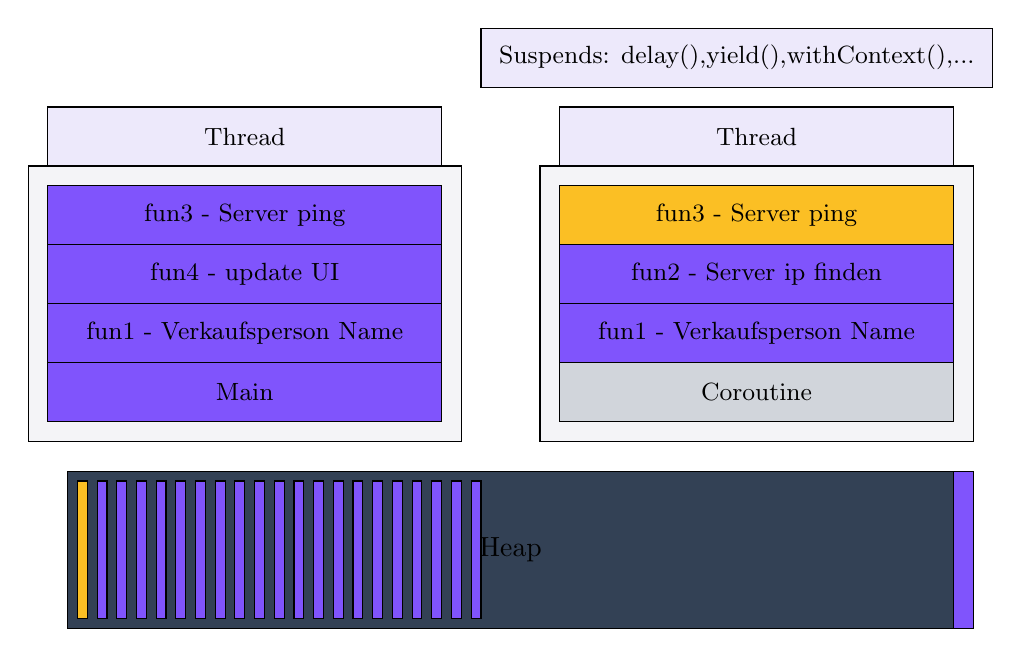
\begin{tikzpicture}
  
%linker Thread
\draw[fill = bgcolor] (0.25,5) rectangle +(5,0.75) node[midway] {\small Thread};

\draw[fill = bgcoloralt] (0,1.5) rectangle +(5.5,3.5) node[midway] {\small Stack};

\uncover<1->{\draw[fill = basecolor] (0.25,1.75) rectangle +(5,0.75) node[midway] {\small Main};}
%rechter Thread
\uncover<3->{

\draw[fill = bgcolor] (6.75,5) rectangle +(5,0.75) node[midway] {\small Thread};

\draw[fill = bgcoloralt] (6.5,1.5) rectangle +(5.5,3.5) node[midway] {\small Stack};

}
\iffalse
\uncover<2>{
\draw[fill = bgcolor] (6.5,6.5) rectangle +(5.75,-7.25);
\node at (9.25,6) {\huge -Unterprozess};
\node at (9.25,5) {\huge -Besteht aus:};
\draw[fill = bgcoloralt] (6.625,4.5) rectangle +(5.5,-3);
\node at (9.35,4) {\huge Stack (Pointer)};
\node at (9.35,3) {\huge Instruction Pointer};
%\node at (9.5,2) {\huge };
\node at (9.25,1) {\huge -OS Lastig};

}

\uncover<3-5>{
\draw[fill = basecolor] (0.25,2.5) rectangle +(5,0.75) node[midway] {\small fun1};
}
\uncover<3-5>{
\draw[fill = basecolor] (0.25,3.25) rectangle +(5,0.75) node[midway] {\small fun2};
}
\uncover<4>{
\draw[fill = basecolor] (0.25,4) rectangle +(5,0.75) node[midway] {\small  cast Thread};
}
\uncover<5>{

\draw[fill = basecolor] (6.5+0.25,1.75) rectangle +(5,0.75) node[midway] {\small fun3};

\draw[fill = basecolor] (6.5+0.25,2.5) rectangle +(5,0.75) node[midway] {\small fun4};
\draw[fill = basecolor] (6.5+0.25,3.25) rectangle +(5,0.75) node[midway] {\small fun5};
%\draw[fill = basecolor] (6.5+0.25,4) rectangle +(5,0.75) node[midway] {\small  fun3 - Server ping};


}

\uncover<6>{
\draw[fill = altbasecolor] (3.5,1.125) rectangle +(5.25,-2) node[midway] {CPU};
\draw[fill = basecolor] (3.75,1) rectangle +(4.75,-0.5) node[midway] {\small fun5 };
\draw[fill = basecolor] (3.75,0.375) rectangle +(4.75,-0.5) node[midway] {\small fun4};
\draw[fill = basecolor] (3.75,-0.25) rectangle +(4.75,-0.5) node[midway] {\small fun3};
}
\fi
%ab hier
\uncover<2>{
\draw[fill = basecolor] (0.25,2.5) rectangle +(5,0.75) node[midway] {\small launch Coroutine};
\draw[fill = basecolor!60] (6.5+0.25,2.5) rectangle +(2.5,0.75) node[midway] {\small launch\{\}};
\draw[fill = basecolor!60] (9+0.25,2.5) rectangle +(2.5,0.75) node[midway] {\small async\{\}};
}

\uncover<3-6>{
\draw[fill = basecolor] (6.5+0.25,1.75) rectangle +(5,0.75) node[midway] {\small Coroutine};
}
\uncover<4-6>{

\draw[fill = basecolor] (6.5+0.25,2.5) rectangle +(5,0.75) node[midway] {\small fun1 - Verkaufsperson Name};
\draw[fill = basecolor] (6.5+0.25,3.25) rectangle +(5,0.75) node[midway] {\small fun2 - Server ip finden};
\draw[fill = basecolor] (6.5+0.25,4) rectangle +(5,0.75) node[midway] {\small  fun3 - Server ping};
}

\uncover<5-6>{

\draw[fill = bgcolor] (5.75,6) rectangle +(6.5,0.75) node[midway] {\small Suspends: delay(),yield(),withContext(),...};

}

\uncover<6>{
\draw[fill = popcolor] (6.5+0.25,4) rectangle +(5,0.75) node[midway] {\small  fun3 - Server ping};
%\draw[fill = popcolor] (6.5+0.25,2.5) rectangle +(5,0.75) node[midway] {\small fun1 - Verkaufsperson Name};
\draw[fill = altbgcoloralt] (6.5+0.25,1.75) rectangle +(5,0.75) node[midway] {\small Coroutine};
}

\uncover<7>{
\draw[fill = basecolor] (6.5,1.125) rectangle +(5.5,-2);
%\fill[basecolor] (6.5+0.125,0.6) rectangle +(2,0.5) %node[midway] {\small Coroutine};
\node at (7.5+0.125,1-0.15) {\texttt{Coroutine:}};
\node at (7.5+0.125,1-0.55) {Variablen:};
\node at (7.5+0.125+3,1-0.55) {Name,Ip};
\node at (7.5+0.125,1-0.95) {State:};
\node at (7.5+0.125+3,1-0.95) {1};
\node at (7.5+0.125,1-1.35) {Path:};
\node at (7.5+0.125+3,1-1.35) {fun1-fun2-fun3};
}
\uncover<8-14>{
\draw[fill = altbasecolor] (0.5,1.125) rectangle +(6+5.25,-2) node[midway] {Heap};
\draw[fill = basecolor] (0.625,1.0) rectangle +(0.125,-1.75);
}
\uncover<9-14>{
\foreach \x in {0,0.25,...,5}{
\draw[fill = basecolor] (0.625+\x,1.0) rectangle +(0.125,-1.75);
}
}

\uncover<10>{
\draw[fill = popcolor] (0.625,1.0) rectangle +(0.125,-1.75);

}
\uncover<11>{
\draw[fill = basecolor] (0.25,4) rectangle +(5,0.75) node[midway] {\small  fun3 - Server ping};
}
\uncover<11-12>{
\draw[fill = basecolor] (0.25,3.25) rectangle +(5,0.75) node[midway] {\small fun2 - Server ip finden};}
\uncover<11-13>{
\draw[fill = basecolor] (0.25,2.5) rectangle +(5,0.75) node[midway] {\small fun1 - Verkaufsperson Name};}

\uncover<13>{
\draw[fill = basecolor] (0.25,3.25) rectangle +(5,0.75) node[midway] {\small fun4 - update UI}; 
}




  \end{tikzpicture}
\end{frame}

\begin{frame}{Android: Coroutines: Beispiel}
\begin{center}
\iffalse
    Multithreading mit Coroutines\\
    Single Thread\\
    Multithreading\\
    \fi
    Beispiel Coroutines
\end{center}
\end{frame}
\iffalse
\begin{frame}{Android: Coroutines: Beispiel}

%\begin{center}
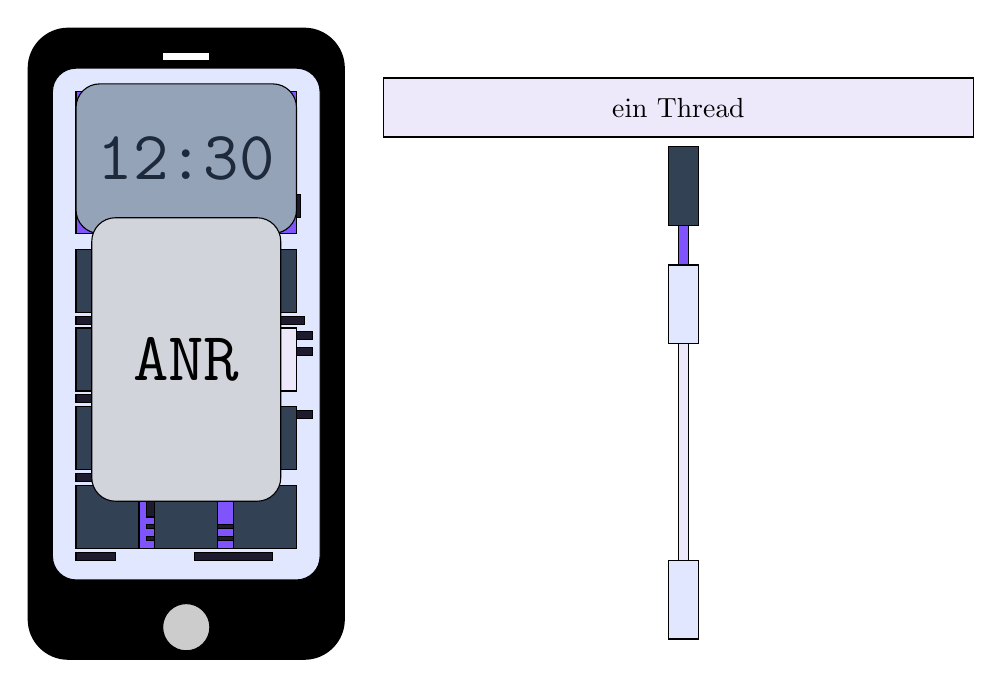
\begin{tikzpicture}

% Phone body
\draw[fill = black, rounded corners=0.5cm, thick] (0,0) rectangle (4,8);

% Screen area

\uncover<1>{\draw[fill=basecolor, rounded corners=0.3cm] (0.3,1) rectangle (3.7,7.5);}
\uncover<2,8->{\draw[fill=bgcolor, rounded corners=0.3cm] (0.3,1) rectangle (3.7,7.5);}
\uncover<3-7>{\draw[fill=altbgcolor, rounded corners=0.3cm] (0.3,1) rectangle (3.7,7.5);}

% Speaker
\draw[fill=white] (1.7,7.6) rectangle (2.3,7.7);

% Home button (circle)
\draw[fill=black!20] (2,0.4) circle (0.3);

% App squares (3x4 grid)
\visible<1>{

      % \pgfmathsetmacro{\randnum}{int(random(0,10))*0.1}; 
  \draw[fill = secondarycolor] (0.6,5.4) rectangle +(1.5,1.5);
  \draw[fill = textcolor] (2.2,6.4) rectangle +(1,0.4);
  \draw[fill = textcolor] (2.2,5.6) rectangle +(1.25,0.3);
  \foreach \x in {0,1.5}{
    \foreach \y in {0,0.2,...,3.8} {
        \pgfmathsetmacro{\num}{random(0,10)*0.1};
        \draw[fill = textcolor] (0.6+\x,\y+1.25) rectangle +(1.5-\num,0.1);
    }
  }
}


\uncover<2,8->{
\foreach \x in { 0.6} { %{0.6, 1.6, 2.6}
  \foreach \y in {1.4, 2.4, 3.4, 4.4, 5.4, 6.4} {
    \draw[fill=basecolor] (\x,\y) rectangle +(2.8,0.8);
    \draw[fill=secondarycolor] (\x+0.1,\y+0.1) rectangle +(0.6,0.6);
    \draw[fill = textcolor] (\x+0.9,\y+0.1) rectangle +(1.8,0.05);
    \draw[fill = textcolor] (\x+0.9,\y+0.25) rectangle +(1.8,0.05);
    \draw[fill = textcolor] (\x+0.9,\y+0.4) rectangle +(0.9,0.2);
  }
}
}
\uncover<4->{\node[draw,fill = bgcolor, minimum width=7.5cm, minimum height=0.75cm, align=center] at (8.25,7) {ein Thread};}
\uncover <4->{
\draw [fill = basecolor] (8.25,6.5) rectangle +(0.125,-6);

}
\uncover<5-7>{ %running process

\draw [fill = bgcolor] (8.25,4.5) rectangle +(0.125,-4);
\draw [fill = altbgcolor] (8.125,5) rectangle +(0.375,-1);
}
\uncover<6,7>{ %paused process
\draw [fill = altbasecolor] (8.125,6.5) rectangle +(0.375,-1);
}


\uncover<8>{

%\draw [fill = bgcolor] (8.25,4.5) rectangle +(0.125,-4);
\draw [fill = altbgcolor] (8.125,1.25) rectangle +(0.375,-1);
}
\uncover<3-7>{
\foreach \x in {0.6, 1.6, 2.6} {
  \foreach \y in {1.4, 2.4, 3.4, 4.4} {
    \draw[fill=altbasecolor] (\x,\y) rectangle +(0.8,0.8);
  }
}

\draw[fill=altpopcolor] (2.6,3.4) rectangle +(0.8,0.8);
%\draw[fill=altsecondarycolor]; 
\draw[fill=altsecondarycolor, rounded corners=0.3cm] (0.6,5.4) rectangle +(2.8,1.9) node[midway] { \Huge\texttt{\textcolor{alttextcolor}{12:30}}};
}
\uncover<7>{
%ANRs
\draw [fill = altbgcoloralt, rounded corners=0.3cm] (0.8,2) rectangle +(2.4,3.6) node[midway] {\Huge\texttt{ANR}};
}
\end{tikzpicture}
%\end{center}

  
\end{frame}
\begin{frame}{Android: Coroutines: Beispiel}
  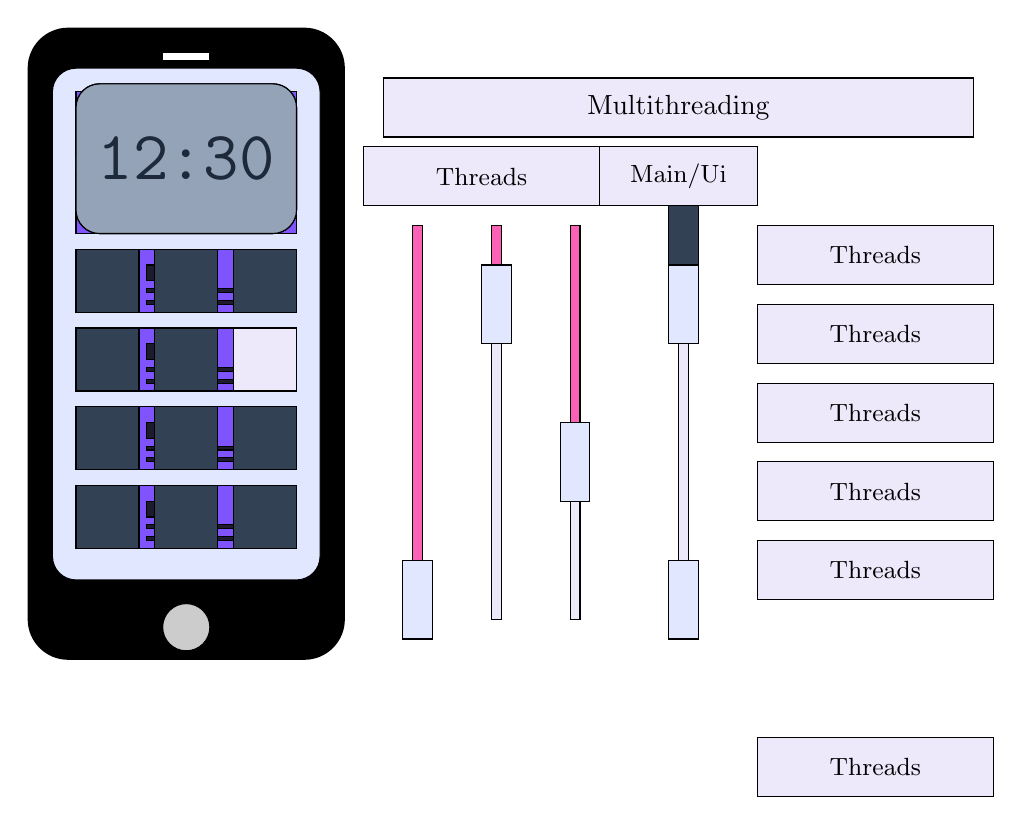
\begin{tikzpicture}

% Phone body
\draw[fill = black, rounded corners=0.5cm, thick] (0,0) rectangle (4,8);

% Screen area


\uncover<6->{\draw[fill=bgcolor, rounded corners=0.3cm] (0.3,1) rectangle (3.7,7.5);}
\uncover<1-5>{\draw[fill=altbgcolor, rounded corners=0.3cm] (0.3,1) rectangle (3.7,7.5);}

% Speaker
\draw[fill=white] (1.7,7.6) rectangle (2.3,7.7);

% Home button (circle)
\draw[fill=black!20] (2,0.4) circle (0.3);




\uncover<6->{
\foreach \x in { 0.6} { %{0.6, 1.6, 2.6}
  \foreach \y in {1.4, 2.4, 3.4, 4.4, 5.4, 6.4} {
    \draw[fill=basecolor] (\x,\y) rectangle +(2.8,0.8);
    \draw[fill=secondarycolor] (\x+0.1,\y+0.1) rectangle +(0.6,0.6);
    \draw[fill = textcolor] (\x+0.9,\y+0.1) rectangle +(1.8,0.05);
    \draw[fill = textcolor] (\x+0.9,\y+0.25) rectangle +(1.8,0.05);
    \draw[fill = textcolor] (\x+0.9,\y+0.4) rectangle +(0.9,0.2);
  }
}
}

\uncover<1->{\node[draw,fill = bgcolor, minimum width=7.5cm, minimum height=0.75cm, align=center] at (8.25,7) {Multithreading};}
\uncover <2->{
\draw [fill = basecolor] (8.25,5.5) rectangle +(0.125,-5);

}
\uncover<4>{ %paused process
\draw [fill = altbasecolor] (8.125,6) rectangle +(0.375,-1);
}
\uncover <2->{
\draw[fill = bgcolor] (7.25,5.75) rectangle +(2,0.75) node[midway] {\small Main/Ui};


}
\uncover<3-5>{ %running process

\draw [fill = bgcolor] (8.25,4.5) rectangle +(0.125,-4);
\draw [fill = altbgcolor] (8.125,5) rectangle +(0.375,-1);
}


\uncover<5>{

%\draw [fill = bgcolor] (8.25,4.5) rectangle +(0.125,-4);
%\draw [fill = altbgcolor] (8.125,1.25) rectangle +(0.375,-1);
}
\uncover<5->{
\draw[fill = bgcolor] (4.25,5.75) rectangle +(3,0.75) node[midway] {\small Threads};
%\draw [fill = basecolor] (8 ,5.5) rectangle +(0.125,-5);
\draw [fill = defaultcolor] (6.75+0.125,5.5) rectangle +(0.125,-5);
\draw [fill = defaultcolor] (5.75+0.125 ,5.5) rectangle +(0.125,-5);
\draw [fill = defaultcolor] (4.75+0.125,5.5) rectangle +(0.125,-5);


\draw [fill = bgcolor] (6.75+0.125,2.5) rectangle +(0.125,-2);
\draw [fill = altbgcolor] (6.75,3) rectangle +(0.375,-1);


\draw [fill = bgcolor] (5.75+0.125,4.5) rectangle +(0.125,-4);
\draw [fill = altbgcolor] (5.75,5) rectangle +(0.375,-1);

\draw [fill = altbgcolor] (4.75,1.25) rectangle +(0.375,-1);
}
\uncover<6->{
\draw [fill = altbgcolor] (8.125,1.25) rectangle +(0.375,-1);


}
\uncover<1-5>{
\foreach \x in {0.6, 1.6, 2.6} {
  \foreach \y in {1.4, 2.4, 3.4, 4.4} {
    \draw[fill=altbasecolor] (\x,\y) rectangle +(0.8,0.8);
  }
  \draw[fill=altpopcolor] (2.6,3.4) rectangle +(0.8,0.8);
%\draw[fill=altsecondarycolor]; 
\draw[fill=altsecondarycolor, rounded corners=0.3cm] (0.6,5.4) rectangle +(2.8,1.9) node[midway] { \Huge\texttt{\textcolor{alttextcolor}{12:30}}};
}
}
\uncover<7>{
\draw[fill = bgcolor] (9.25,4.75) rectangle +(3,0.75) node[midway] {\small Threads};
\draw[fill = bgcolor] (9.25,3.75) rectangle +(3,0.75) node[midway] {\small Threads};
\draw[fill = bgcolor] (9.25,2.75) rectangle +(3,0.75) node[midway] {\small Threads};
\draw[fill = bgcolor] (9.25,1.75) rectangle +(3,0.75) node[midway] {\small Threads};
\draw[fill = bgcolor] (9.25,0.75) rectangle +(3,0.75) node[midway] {\small Threads};
\draw[fill = bgcolor] (9.25,-1.75) rectangle +(3,0.75) node[midway] {\small Threads};
}


\end{tikzpicture}
\end{frame}
\fi
\begin{frame}{Android: Coroutines: Beispiel}
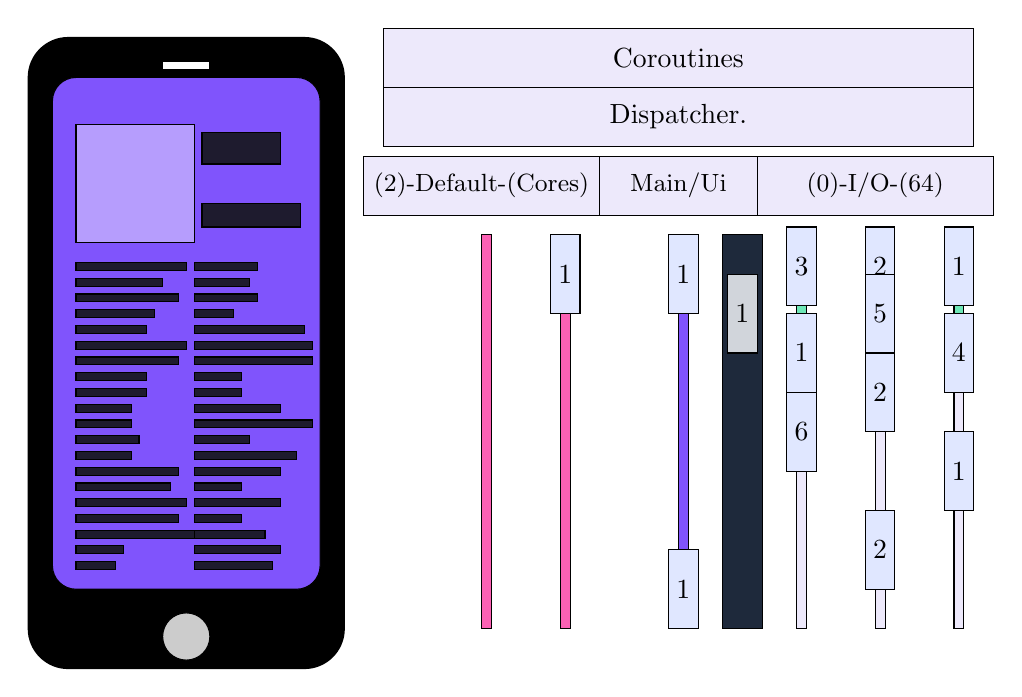
\begin{tikzpicture}


% Phone body
\draw[fill = black, rounded corners=0.5cm, thick] (0,0) rectangle (4,8);

% Screen area
\uncover<1-5>{\draw[fill=altbgcolor, rounded corners=0.3cm] (0.3,1) rectangle (3.7,7.5);


\foreach \x in {0.6, 1.6, 2.6} {
  \foreach \y in {1.4, 2.4, 3.4, 4.4} {
    \draw[fill=altbasecolor] (\x,\y) rectangle +(0.8,0.8);
  };
  \draw[fill=altpopcolor] (2.6,3.4) rectangle +(0.8,0.8);
%\draw[fill=altsecondarycolor]; 
\draw[fill=altsecondarycolor, rounded corners=0.3cm] (0.6,5.4) rectangle +(2.8,1.9) node[midway] { \Huge\texttt{\textcolor{alttextcolor}{12:30}}};
}




};
\uncover<6-9>{
\draw[fill=bgcolor, rounded corners=0.3cm] (0.3,1) rectangle (3.7,7.5);

\foreach \x in { 0.6} { %{0.6, 1.6, 2.6}
  \foreach \y in {1.4, 2.4, 3.4, 4.4, 5.4, 6.4} {
    \draw[fill=basecolor] (\x,\y) rectangle +(2.8,0.8);
    \draw[fill=secondarycolor] (\x+0.1,\y+0.1) rectangle +(0.6,0.6);
    \draw[fill = textcolor] (\x+0.9,\y+0.1) rectangle +(1.8,0.05);
    \draw[fill = textcolor] (\x+0.9,\y+0.25) rectangle +(1.8,0.05);
    \draw[fill = textcolor] (\x+0.9,\y+0.4) rectangle +(0.9,0.2);
  };
}

};
\visible<10->{
\draw[fill=basecolor, rounded corners=0.3cm] (0.3,1) rectangle (3.7,7.5);
    % \pgfmathsetmacro{\randnum}{int(random(0,10))*0.1}; 
  \draw[fill = secondarycolor] (0.6,5.4) rectangle +(1.5,1.5);
  \draw[fill = textcolor] (2.2,6.4) rectangle +(1,0.4);
  
  \foreach \x in {0,1.5}{
    \foreach \y in {0,0.2,...,3.8} {
        \pgfmathsetmacro{\num}{random(0,10)*0.1};
        \draw[fill = textcolor] (0.6+\x,\y+1.25) rectangle +(1.5-\num,0.1);
    };
  };
};
\uncover<11->{
\draw[fill = textcolor] (2.2,5.6) rectangle +(1.25,0.3);
};
% Speaker
\draw[fill=white] (1.7,7.6) rectangle (2.3,7.7);

% Home button (circle)
\draw[fill=black!20] (2,0.4) circle (0.3);


%right side slide
\uncover<1->{\node[draw,fill = bgcolor, minimum width=7.5cm, minimum height=0.75cm, align=center] at (8.25,7.75) {Coroutines};}
\uncover<2->{
\node[draw,fill = bgcolor, minimum width=7.5cm, minimum height=0.75cm, align=center] at (8.25,7) {Dispatcher.};
%Default
\draw[fill = bgcolor] (4.25,5.75) rectangle +(3,0.75) node[midway] {\small (2)-Default-(Cores)};
%\draw [fill = basecolor] (8 ,5.5) rectangle +(0.125,-5);
\draw [fill = defaultcolor] (6.75+0,5.5) rectangle +(0.125,-5);
\draw [fill = defaultcolor] (5.75+0 ,5.5) rectangle +(0.125,-5);


%Main
\draw [fill = basecolor] (8.25,5.5) rectangle +(0.125,-5);
\draw[fill = bgcolor] (7.25,5.75) rectangle +(2,0.75) node[midway] {\small Main/Ui};

%I/O
\draw[fill = bgcolor] (9.25,5.75) rectangle +(3,0.75) node[midway] {\small (0)-I/O-(64)};
%\draw [fill = basecolor] (8 ,5.5) rectangle +(0.125,-5);
%\draw [fill = bgcolor] (6.75+0.125,2.5) rectangle +(0.125,-2);
%\draw [fill = altbgcolor] (6.75,3) rectangle +(0.375,-1);


%\draw [fill = bgcolor] (5.75+0.125,4.5) rectangle +(0.125,-4);
%\draw [fill = altbgcolor] (5.75,5) rectangle +(0.375,-1);

%\draw [fill = altbgcolor] (4.75,1.25) rectangle +(0.375,-1);
};
\uncover<3->{
%\draw [fill = defaultcolor] (4.75+0,5.5) rectangle +(0.125,-5);


\draw [fill = iocolor] (6.75+5,5.5) rectangle +(0.125,-5);
\draw [fill = iocolor] (5.75+5 ,5.5) rectangle +(0.125,-5);
\draw [fill = iocolor] (4.75+5,5.5) rectangle +(0.125,-5);

};
\uncover<3>{
\draw [fill = altbgcolor] (6.75+5-0.125,5.6) rectangle +(0.375,-1) node[midway] {1};
\draw [fill = altbgcolor] (5.75+5-0.125,5.6) rectangle +(0.375,-1) node[midway] {2};
\draw [fill = altbgcolor] (4.75+5-0.125,5.6) rectangle +(0.375,-1) node[midway] {3};

};
\uncover<4>{

\draw [fill = bgcolor] (6.75+5,2.5) rectangle +(0.125,-2);
\draw [fill = altbgcolor] (6.75+5-0.125,3) rectangle +(0.375,-1) node[midway] {1};
\draw [fill = bgcolor] (5.75+5,3.5) rectangle +(0.125,-3);
\draw [fill = altbgcolor] (5.75+5-0.125,4) rectangle +(0.375,-1) node[midway] {2};
\draw [fill = bgcolor] (4.75+5,4) rectangle +(0.125,-3.5);
\draw [fill = altbgcolor] (4.75+5-0.125,4.5) rectangle +(0.375,-1) node[midway] {3};

};

\uncover<5>{

\draw [fill = bgcolor] (6.75+5,4) rectangle +(0.125,-3.5);
\draw [fill = altbgcolor] (6.75+5-0.125,4.5) rectangle +(0.375,-1) node[midway] {4};
\draw [fill = bgcolor] (5.75+5,4.5) rectangle +(0.125,-4);
\draw [fill = altbgcolor] (5.75+5-0.125,5) rectangle +(0.375,-1) node[midway] {5};
\draw [fill = bgcolor] (4.75+5,3) rectangle +(0.125,-2.5);
\draw [fill = altbgcolor] (4.75+5-0.125,3.5) rectangle +(0.375,-1) node[midway] {6};
%paused coroutines
\draw[fill = alttextcolor] (4+5-0.25+0.0625,5.5) rectangle +(0.5,-5); %node[midway] {3};
\draw [fill = altbgcoloralt] (4+5-0.125,5) rectangle +(0.375,-1) node[midway] {3};
\draw [fill = altbgcoloralt] (4+5-0.125,3.5) rectangle +(0.375,-1) node[midway] {2};
\draw [fill = altbgcoloralt] (4+5-0.125,2) rectangle +(0.375,-1) node[midway] {1};

};
\uncover<6>{

%\draw [fill = bgcolor] (6.75+5,2.5) rectangle +(0.125,-2);
\draw [fill = altbgcolor] (6.75+5-0.125,3) rectangle +(0.375,-1) node[midway] {1};
%\draw [fill = bgcolor] (5.75+5,3.5) rectangle +(0.125,-3);
\draw [fill = altbgcolor] (5.75+5-0.125,4) rectangle +(0.375,-1) node[midway] {2};
%\draw [fill = bgcolor] (4.75+5,4) rectangle +(0.125,-3.5);
\draw [fill = altbgcolor] (8.25-0.125,1.5) rectangle +(0.375,-1) node[midway] {3};
%paused coroutines
\draw[fill = alttextcolor] (4+5-0.25+0.0625,5.5) rectangle +(0.5,-5); %node[midway] {3};
\draw [fill = altbgcoloralt] (4+5-0.125,5) rectangle +(0.375,-1) node[midway] {6};
\draw [fill = altbgcoloralt] (4+5-0.125,3.5) rectangle +(0.375,-1) node[midway] {5};
\draw [fill = altbgcoloralt] (4+5-0.125,2) rectangle +(0.375,-1) node[midway] {4};

};
\uncover<7>{


%\draw [fill = bgcolor] (4.75+5,4) rectangle +(0.125,-3.5);
\draw [fill = altbgcolor] (5.75+5-0.125,4) rectangle +(0.375,-1) node[midway] {2};
\draw [fill = altbgcolor] (4.75+5-0.125,4.5) rectangle +(0.375,-1) node[midway] {1};


};
\uncover<8>{

\draw[fill = alttextcolor] (4+5-0.25+0.0625,5.5) rectangle +(0.5,-5); %node[midway] {3};
%\draw [fill = bgcolor] (5.75+5,3.5) rectangle +(0.125,-3);
\draw [fill = altbgcolor] (5.75+5-0.125,2) rectangle +(0.375,-1) node[midway] {2};
\draw [fill = altbgcoloralt] (4+5-0.125,5) rectangle +(0.375,-1) node[midway] {1};


};
\uncover<9>{
\draw [fill = altbgcolor] (8.25-0.125,5.5) rectangle +(0.375,-1) node[midway] {2};
\draw [fill = altbgcolor] (6.75-0.125,5.5) rectangle +(0.375,-1) node[midway] {1};
};
\uncover<10>{
\draw [fill = altbgcolor] (8.25-0.125,5.5) rectangle +(0.375,-1) node[midway] {1};
\draw [fill = altbgcolor] (8.25-0.125,1.5) rectangle +(0.375,-1) node[midway] {2};

};
\uncover<11>{
%\draw [fill = altbgcolor] (8.25-0.125,5.5) rectangle +(0.375,-1) node[midway] {1};
\draw [fill = altbgcolor] (8.25-0.125,1.5) rectangle +(0.375,-1) node[midway] {1};

};
\end{tikzpicture}
\end{frame}

\begin{frame}{Zusammenfassung} %Der gesamten Präsentation
  \begin{itemize}
    \item Moderne Programmiersprache mit präziser Syntax und innovativen Features.
    \item Verbesserte Klassenstrukturen und Null-Sicherheit.
    \item Nahtlose Interoperabilität mit Java
    \item Multiplattform-Entwicklung (Android)
  \end{itemize}
  \vspace{1cm}
  \pause\textbf{Aussicht:}
  \begin{itemize}
    \item Erweiterte Features: Smart Casts, Delegation, Destructuring \ldots
    \item Unterstützung funktionaler Programmierparadigmen
  \end{itemize}
      %Notes: Koltin ist eine leistungstarke alternative zu Java
\end{frame}
  

\end{document}